%\documentclass[compress]{beamer}
\documentclass[compress,handout]{beamer}

%%%%% PREAMBLE %%%%%

% we want to draw diagrams (turns out not like this though)
\usepackage{tikz}

% figures in a presentation look better without "Figure"
\usepackage{caption}
\captionsetup[figure]{labelformat=empty}

% for Idris syntax highlighting
\usepackage[styles]{idrislang}

% slide url at the end
\usepackage{hyperref}
\hypersetup{
  colorlinks=true,
  urlcolor=purple
}

% N.B. For some reason, things don't build without this...
\usepackage{todonotes}
\setuptodonotes{inline} % for things to work nicely with beamer

%\usetheme{Zurich}  % doesn't work for some reason
%\usetheme{Flip}
\usetheme{metropolis}

\title{TBD}
\subtitle{Uniting the Spectrum of Verification}

\author{Thomas Ekstr{\" o}m Hansen}
\date{6\textsuperscript{th} March 2024}

\definecolor{staBlue}{HTML}{00539b}
\definecolor{staMidGreen}{HTML}{00853f}
\definecolor{staDarkGreen}{HTML}{005953}
\setbeamercolor{frametitle}{bg=staDarkGreen}


%%%%% DOCUMENT %%%%%

\begin{document}

\maketitle


\begin{frame}
  \frametitle{Overview}

  \begin{itemize}
    \item<1-> Many systems exhibit Finite State Machine (FSM)-like behaviour
    \begin{itemize}
      \item<1-> These can be neatly modelled with Dependent Types
    \end{itemize}
    \item<2-> ATM example of this from Edwin Brady's ``Type Driven
              Development with Idris'' book
    \begin{itemize}
      \item<2-> Turns out this example is subtly incorrect
    \end{itemize}
    \item<3-> How can we spot this? Can we increase confidence in our type-level
              modelling without having to ``just get it right''?
    \item<4-> Spoilers: How does QuickCheck fit in with dependent types?
    \item<5-> No panacea, but we can hopefully catch errors faster and have some
              guarantees that our model behaves as intended.
  \end{itemize}

\end{frame}


\begin{frame}
  \frametitle{The ATM state machine}

  \begin{center}
  \begin{figure}
    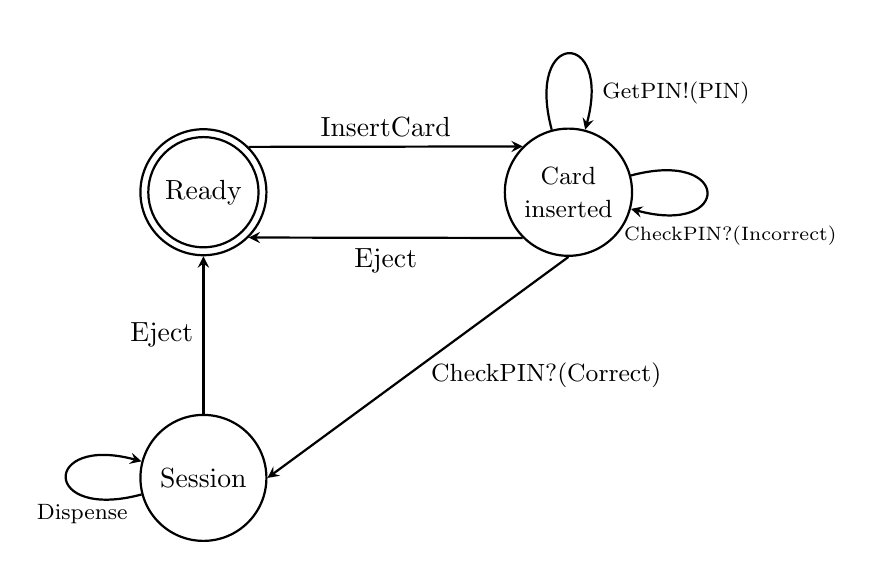
\begin{tikzpicture}[> = stealth, thick,
                        roundnode/.style={circle, draw=black!100, minimum size=16mm},
                        node distance=2cm and 3cm]
      % ATM states %
      \node [circle, draw=black!100, minimum size=14mm] {} ;
      \node[roundnode] (st-ready) {Ready} ;
      \node[roundnode] (st-card) [right=of st-ready, align=center] {\small Card\\\small inserted} ;
      \node[roundnode] (st-session) [below=of st-ready] {Session} ;

      % Arrows %
      \draw [->] (st-ready.north east) -- (st-card.north west)
            node [above, midway] {InsertCard} ;

      \draw [->] (st-card.south west) -- (st-ready.south east)
            node [below, midway] {Eject} ;
      \draw [->] (st-card.south) -- (st-session.east)
            node [right, midway, xshift=1pt, yshift=-1mm] {\small CheckPIN?(Correct)} ;

      \draw [->] (st-session.north) -- (st-ready.south)
            node [left, midway] {Eject} ;

      % Lööps %
      \draw [->] (st-card) to[loop above]
            node [right, xshift=3mm, yshift=-5mm] {\footnotesize GetPIN!(PIN)}
            () ;
      \draw [->] (st-card) to[loop right]
            node [below, xshift=3mm, yshift=-3mm] {\scriptsize CheckPIN?(Incorrect)}
            () ;
      \draw [->] (st-session) to[loop left]
            node [below, xshift=2mm, yshift=-2mm] {\footnotesize Dispense} () ;
    \end{tikzpicture}

    \caption{State machine of an ATM}
  \end{figure}
  \end{center}

\end{frame}


\begin{frame}
  \frametitle{Finite State Monads}

  % TODO: try to get this nicer via Katla?
  \vspace*{-3mm}
  \idrisinput{ATM.idr}
\end{frame}


%% FIXME: is this relevant for the talk?
%% \begin{frame}
%%   \frametitle{There are patterns in these}
%%   \todo{Is this relevant for the talk?}
%%
%%   \begin{itemize}
%%     \item The \texttt{Bind}, \texttt{Seq}, and \texttt{Pure} commands are always
%%           the same
%%     \begin{enumerate}
%%       \item Given a state, a result, and what to do next, can bind from state 1
%%             to state 3
%%       \item Trivially so if the result is \texttt{Unit}
%%       \item And if we have a value, we can shove it in a state as long as the
%%             state function accepts something of the value's type
%%     \end{enumerate}
%%     \item State-names map to \texttt{CMD} constructors
%%     \item And dependent states' pattern-matches can be lifted to
%%           \texttt{<...>Res} types
%%   \end{itemize}
%%
%% \end{frame}


\begin{frame}
  \frametitle{How do you generate a dependent type?}

  \begin{itemize}
    \item QuickCheck's bread and butter is \texttt{Arbitrary}
    \begin{itemize}
      \item Define how to generate an instance of a type, given some
            pseudorandom number generator state
      \item Reasonably straightforward for random numbers, picking an element,
            and structures where the type of the constructors are known at
            generation-time
    \end{itemize}
    \item However, our types are \textit{dependent}
    \item So we cannot know the exact type at generation time
    \begin{itemize}
      \item We can know \textit{a} type, but not all. For example, \texttt{Vect
            5 Nat} is fine
      \item The problem is \texttt{Vect n Nat}
      \item Or even \texttt{Arbitrary t $=>$ Vect n t}
    \end{itemize}
  \end{itemize}

\end{frame}


\begin{frame}[fragile]
  \frametitle{Arbitrary dependent types}
  
  \begin{itemize}
    \item The solution is more dependent types!
    \item Specifically: dependent pairs

    \vspace*{-6mm}
    \begin{idrislisting}
record DPair a (p : a -> Type) where
  constructor MkDPair
  fst : a
  snd : p fst
    \end{idrislisting}
    \vspace*{-3mm}

    \item As long as we know how to generate an {\textasciigrave
          \texttt{Arbitrary a}\textasciigrave}, we can generate an
          {\textasciigrave\texttt{Arbitrary (x : a ** p x)}\textasciigrave}
    \item Coming back to vectors:
    \vspace*{-6mm}
    \begin{idrislisting}
Arbitrary a => Arbitrary (n : Nat ** Vect n a)
    \end{idrislisting}
    \begin{itemize}
    \vspace*{-2mm}

      \item (The \texttt{**} syntax is sugar for \texttt{DPair}/\texttt{MkDPair}
            depending on the context)
    \end{itemize}
  \end{itemize}

\end{frame}


\begin{frame}[fragile]  % <--- N.B. `fragile` required for listing to work
  \frametitle{Using types only gets you part of the way there}

  \begin{columns}
  \begin{column}{0.47\framewidth}
    {\color{red} Rejected by the compiler:}
    \vspace*{-3mm}
    \begin{idrislisting}[basicstyle=\ttfamily\scriptsize]
badProg : CMD ()
            Ready (const Ready)
badProg =
  do InsertCard
     pin <- GetPIN
     Correct <- CheckPIN pin
       | Incorrect => InsertCard
     amt <- GetAmount
     Dispense amt 
     -- we never EjectCard
    \end{idrislisting}
  \end{column}

  \pause  % first show the bad, then the dubious

  \hspace*{-0.6mm}
  \vrule{}

  \begin{column}{0.53\framewidth}
    {\color{orange} Accepted by the compiler:}
    \vspace*{-3mm}
    \begin{idrislisting}[basicstyle=\ttfamily\scriptsize]
atmProg : CMD ()
            Ready (const Ready)
atmProg =
  do InsertCard
     pin <- GetPIN
     _ <- CheckPIN pin
     _ <- CheckPIN pin
     _ <- CheckPIN pin
     _ <- CheckPIN pin
     <...>
     amt <- GetAmount
     Dispense amt 
     EjectCard
    \end{idrislisting}
    \vspace*{-1cm}
  \end{column}
  \end{columns}
\end{frame}


\begin{frame}
  \frametitle{Disadvantages of the \texttt{CMD}-like approach}

  \begin{itemize}
    \item<1-> Not the most ergonomic
    \begin{itemize}
      \item<2-> It is a Domain Specific Language
      \item<3-> So it needs an interpreter; it is not directly runnable code
      \item<4-> The type declarations can get lengthy
    \end{itemize}
    \item<5-> Composition is currently undefined
    \begin{itemize}
      \item<6-> The theory it builds on does not currently support composition
      \item<7-> But we often want to compose code and functionality
    \end{itemize}
  \end{itemize}
\end{frame}


\begin{frame}[fragile]
  \frametitle{Spectrum of Verification}

  \hspace*{-5mm}  % to fit the bounding box of the tikz diagram
  % ~~probably~~ definitely cursed
  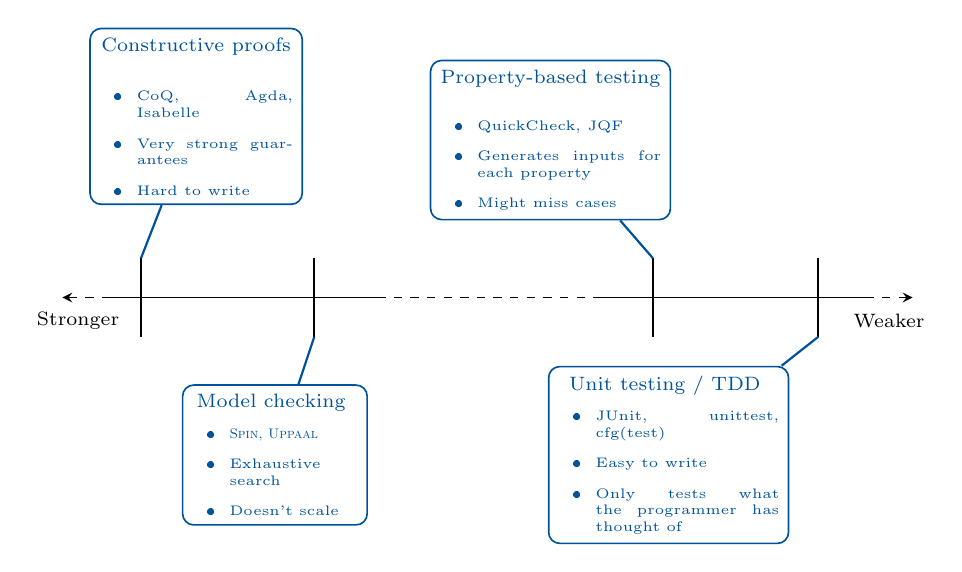
\begin{tikzpicture}[> = stealth, semithick]
    % scale %

    % left half
    \draw [dashed, <-] (-0.2, 0) -- (0.4, 0) ;
    \draw (0.4, 0) -- (3.8, 0) ;

    % middle dashed
    \draw [dashed] (3.8, 0) -- (6.6, 0) ;

    % right half
    \draw (6.6, 0) -- (10, 0) ;
    \draw [dashed, ->] (10, 0) -- (10.6, 0) ;


    % ticks / vertical lines %

    % leftmost tick (constructive proofs)
    \draw<2-> (0.8, -0.5) -- (0.8, 0.5) ;
    
    % tick for model checking
    \draw<3-> (3, -0.5) -- (3, 0.5) ;

    % tick for Quickcheck
    \draw<4-> (7.3, -0.5) -- (7.3, 0.5) ;

    % rightmost tick (unit tests)
    \draw<5-> (9.4, -0.5) -- (9.4, 0.5) ;


    % scale labels %

    \node at (0, -0.3) {\scriptsize Stronger} ;
    \node at (10.3, -0.3) {\scriptsize Weaker} ;


    % text boxes with arrows %

    % constructive proofs
    \node<2->
          [draw, rounded corners,
          text width=7em,
          align=flush center,
          color=staBlue]% 
          at (1.5, 2.3)
          (tbox-prf)
          \bgroup
          \scriptsize
          Constructive proofs
          \vspace*{-2pt}
          \tiny
          % LaTeX looks beautiful and nice
          % Also LaTeX:
          \setlength{\leftmargini}{2em}
          \begin{itemize}%[leftmargin=*]
            \item CoQ, Agda, Isabelle \vspace*{-3pt}
            \item Very strong guarantees \vspace*{-3pt}
            \item Hard to write
          \end{itemize}
          \egroup
          ;
    \draw<2-> [thick, color=staBlue] (tbox-prf) -- (0.8, 0.5) ;

    % model checking
    \node<3->
          [draw, rounded corners,
          text width=6em,
          align=flush center,
          color=staBlue]% 
          at (2.5, -2)
          (tbox-mc)
          \bgroup
          \scriptsize
          Model checking
          \vspace*{-3pt}
          \tiny
          \setlength{\leftmargini}{2em}
          \begin{itemize}%[leftmargin=*]
            \item \textsc{Spin, Uppaal}  \vspace*{-3pt}
            \item Exhaustive search  \vspace*{-3pt}
            \item Doesn't scale
          \end{itemize}
          \egroup
          ;
    \draw<3-> [thick, color=staBlue] (tbox-mc) -- (3, -0.5) ;

    % property-based testing
    \node<4->
          [draw, rounded corners,
          text width=8em,
          align=flush center,
          color=staBlue]% 
          at (6, 2)
          (tbox-qc)
          \bgroup
          \scriptsize
          Property-based testing
          \vspace*{-3pt}
          \tiny
          \setlength{\leftmargini}{2em}
          \begin{itemize}%[leftmargin=*]
            \item QuickCheck, JQF \vspace*{-3pt}
            \item Generates inputs for each property \vspace*{-3pt}
            \item Might miss cases
          \end{itemize}
          \egroup
          ;
    \draw<4-> [thick, color=staBlue] (tbox-qc) -- (7.3, 0.5) ;

    % tdd
    \node<5->
          [draw, rounded corners,
          text width=8em,
          align=flush center,
          color=staBlue]% 
          at (7.5, -2)
          (tbox-tdd)
          \bgroup
          \scriptsize
          Unit testing / TDD
          \vspace*{-3pt}
          \tiny
          \setlength{\leftmargini}{2em}
          \begin{itemize}%[leftmargin=*]
            \item JUnit, unittest, cfg(test) \vspace*{-3pt}
            \item Easy to write \vspace*{-3pt}
            \item Only tests what the programmer has thought of
          \end{itemize}
          \egroup
          ;
    \draw<5-> [thick, color=staBlue] (tbox-tdd) -- (9.4, -0.5) ;

  \end{tikzpicture}

\end{frame}


\begin{frame}
  \frametitle{The eternal problem with verification systems}

  \begin{itemize}
    \item<1-> All verification systems face the same problem: ergonomics
    \item<2-> If the system is not unobtrusive, people are unlikely to use it
    \item<3-> Our hope is that our approach tries to not get in the way by being
              part of the program
      \begin{itemize}
        \item<4-> Compiler and type-system assist you rather than hinder
        \item<5-> Verify as you go along, tuning the strictness as necessary
        \item<6-> Escape hatches provided for prototyping
      \end{itemize}
  \end{itemize}

\end{frame}


\begin{frame}
  \frametitle{Benefits of a multifaceted approach}

  \begin{enumerate}
    \item<1-> Adaptability {\textemdash} right tool for the job
    \item<2-> Speed {\textemdash} can trade speed for level of verification
    \item<3-> \textbf{Coherence} {\textemdash} all done in one system
      \begin{itemize}
        \item<4-> No need to translate to model-checking tool
        \item<5-> Specification lives alongside model lives alongside
                  implementation
        \item<6-> The implementation is just there; it \emph{is} runnable code
        \item<7-> Parts can be verified independently \emph{while} combining into an
                  overall system
      \end{itemize}
  \end{enumerate}

\end{frame}


\begin{frame}
  \frametitle{Conclusion}

  \begin{itemize}
    \item<1-> Many verification tools exist, none of them cover enough on their
              own
    \item<2-> Instead of ``competing'', we combine the systems to work together
    \item<3-> Hopefully this will lead to wider adoption and better whole-system
              soundness
  \end{itemize}

\end{frame}


\begin{frame}
  \frametitle{Questions}

  \begin{center}
    \textcolor<1>{orange}{\Large Questions?}
  \end{center}

\end{frame}

%% TODO
%% \begin{frame}
%%   \frametitle{Slides}
%% 
%%   \begin{center}
%%     \begin{figure}
%%       
\includegraphics[width=0.35\framewidth]{qr-code.png}
%%       \caption{\href{https://github.com/CodingCellist/talks/blob/main/2024-03-06-slps-st-andrews}{github.com/CodingCellist/talks}}
%%     \end{figure}
%%   \end{center}
%% 
%% \end{frame}

\end{document}
